\section{Online Contactless Finger Knuckle Identification}

With RSIL loss, the RFNet \cite{liu2020contactless} can outperform state-of-the-art methods. In the previous section, we have estimated its verification and identification performance on different public finger knuckle database, including within-db and cross-db experiments. As for a completely contactless and online finger knuckle identification, the finger knuckle detector is a very important module for automatically detect and segment finger knuckle region. As for neural network, the current based on YOLO \cite{redmon2016you}, \cite{redmon2017yolo9000}, \cite{redmon2018yolov3}, \cite{bochkovskiy2020yolov4}, \cite{YOLOv5} and R-CNN \cite{girshick2014rich}, \cite{girshick2015fast}, \cite{ren2015faster}, \cite{he2017mask} series object detection and segmentation approaches cannot obtain the angle of finger knuckle and the segmentation with high precision. If we can get the angle of finger knuckle, we can use angle information to align two feature maps for increasing matching accuracy and efficiency. For solving above problems, we use the CSL\cite{yang2020csl} to smooth angular classes for predicting oriented bounding box based on YOLOv5 model for segmenting and getting angle information.

\subsection{Completely Contactless Finger Knuckle Detection}
\subsubsection{ Oriented Bounding Box Based on YOLOv5}
In order to solve the problem of finger knuckle detection in the real world, we choose to use YOLOv5 model because the YOLO series is famous for its fast detection speed and high accuracy. It also provides different variant of YOLOv5 models for different requirements on the inference time and detection accuracy. Especially, the YOLOv5's \cite{YOLOv5} speed can meet our online detection requirements for real-time finger knuckle detection. However, the YOLOv5 just detect horizontal bounding boxes which cannot offer angle information and will segment a lot of background information. In order to solve these above problem, an oriented bounding box will be predicted instead of a horizontal bounding box.

\begin{figure}[ht!]
	\centering
	\begin{subfigure}[b]{0.45\linewidth}
		\centering
		\includegraphics[width=0.6\linewidth]{Figures/five-parameter-definition-finger.png}
		\caption{Five-parameter definition with $180^{\circ}$ angular range.}
	\end{subfigure}
	\begin{subfigure}[b]{0.45\linewidth}
		\centering
		\includegraphics[width=0.7\linewidth]{Figures/CSL-angle.png}
		\caption{Circle smooth label with Gaussian window function.}
	\end{subfigure}
	\caption{Oriented rectangle definition and the circle smooth label method.}
	\label{Long-side&CSL}
\end{figure}


As analyzed in this paper \cite{yang2020csl}, the oriented bounding boxes loss will mainly come from angular periodicity and the exchangeability of edges, if we use the $90^\circ$ OpenCV oriented bounding boxes definition. When use the long side definition of oriented bounding box with $180^\circ$, as shown on the Figure \ref{Long-side&CSL} (a), it can deal with the exchangeability of edges problem. Meanwhile, using classification task to predict angle can make model easier to train when compare to regression. A periodic coding method called Circular Smooth Label (CSL) \cite{yang2020csl} soft coding with Gaussian window function can solve two problems. One is that one-hot cannot distinguish class relationship, and another one is that the predicted angle have periodicity. Formula \ref{CSL Function} $g(x)$ is the window function to smooth one-hot label, and $r$ is a window function of the radius, in the paper $r=6$ can get the best performance. Therefore, we used the Gaussian function for the Equation \ref{CSL Function} window function, a commonly available function, and used a window radius of 6 to smooth the labels. And the period of this function is $180^\circ$, which is the same as the period of the predicted angle, as shown on the Figure \ref{Long-side&CSL} (b).

\begin{equation}
    CSL(x)=
    \begin{cases}
        g(x), &\theta-r<x<r+\theta \\
        0   , &\text{otherwise}
    \end{cases}
    \label{CSL Function}
\end{equation}

The original YOLOv5 loss function can have three components. The formula can be simply written as $Loss = Loss_{bbox} + Loss_{obj} + Loss_{class}$. As for the $Loss_{bbox}$, the YOLOv5 uses the GIOU loss to calculate the loss between predicted bounding boxes and ground truth. Since the oriented bounding box is based on the modification of YOLOv5, only the angle classification loss is added more. So the total loss function is as expressed in Equation \ref{Loss}, with the addition of $Loss_{angle}$ to YOLOv5 loss function. We use the binary cross-entropy to calculate the angle classification loss. In the Equation \ref{Loss_angle}, the $S^2$ is the output grid size, and the $I_{ij}^{obj}$ represents just calculate the loss when object fall in the grid cell.
\begin{equation}
    Loss = Loss_{bbox} + Loss_{obj} + Loss_{class} + Loss_{angle}
    \label{Loss}
\end{equation}
\begin{equation}
    \begin{aligned}
        Loss_{angle} = \sum_{i=0}^{S^2}I_{ij}^{obj}\sum_{a{\in}[0,180)}[\hat{P_i(a)}log(P_i(a)) + (1-\hat{P_i(a)})log(1-P_i(a))]
    \end{aligned}
    \label{Loss_angle}
\end{equation}

\subsubsection{Contactless Finger Knuckle Dataset}
Our task is to detect finger knuckles in the contactless and online scenario, but by understanding current public finger knuckle database, their data are collected at specific conditions such as certain angle, certain light. In this kind of situation, this kind of data cannot represent real images of finger knuckle in real world. In order to address the shortcomings of current public finger knuckle dataset for contactless detection, we use a web crawler to get images from the Unsplash \cite{Unsplash} where the keywords are finger knuckles. The Unsplash is an image site that offers uploads and downloads, and uses a copyright license that allows users to download and use them for free or even for commercial use \cite{unsplashlicense}. We have downloaded 2347 images, there are 738 images without knuckles, and these images can be used as background training, and the rest 1609 images that contain at least one finger knuckle are the positive samples for the network model. In the network training process, we use crawled images, 169 finger knuckle images from the HKPolyU Finger Knuckle Database (V1.0) \cite{fingerknuckledbv1.0}, and 64 finger knuckles images from the HKPolyU Hand Dorsal Database \cite{ContactlessHnadDorsaldb} as for the training set. And we use the rest data as testing set to evaluate performance. The most important part is the data augmentation which contains flip, rotation, resize, translate and mosaic.

\subsubsection{Contactless Finger Knuckle Detection}

\noindent\textbf{Detection Performance}

\noindent
The YOLOv5x, and YOLOv5m model predict horizontal bounding box, while the remaining YOLOv5 model predict oriented bounding box with CSL to smooth angular classification, called YOLOv5-CSL. We can see the performance difference between these variations of the YOLOv5 model from the Table \ref{mAP of different model}. Among the downloaded 2580 images, 100 images were randomly selected as the testing set. The YOLOv5x-CSL can get the highest mAP value with 89.9, especially, the AP of minor finger knuckle can get 90.1. On the contrary, without predicting oriented bounding box, the YOLOv5x detection accuracy is lower 1.6 mAP when compare to YOLOv5x-CSL.

\begin{table}[ht!]
    \centering
    \begin{tabular}{c c c c c c}
        \hline
        Model & \makecell[c]{Total \\ Time/ms\\ (1024x1024)} & \makecell[c]{Number \\of Layers} & \makecell[c]{${mAP}^{val}$\\0.5} & \makecell[c]{AP of\\ Major \\FK} & \makecell[c]{AP of\\ Minor \\FK}\\
        \hline
        YOLOv5x-CSL & 40.9ms & 407 & \textbf{89.9} &\textbf{89.6} & \textbf{90.1} \\
        YOLOv5m-CSL & 23.3ms & 263 & 85.7 & 88.9 & 80.4 \\
        YOLOv5x & 33.3 ms & 407 & 87.3 & 86.5 & 88.0  \\
        YOLOv5m & 12.1ms & 263 & 84.8 & 84.5 & 85.1 \\
        \hline
    \end{tabular}
    \caption{Comparison of the accuracy of the different models of the YOLO series for detecting finger knuckle. The calculated values of mAP were measured at a detection threshold of 0.001 as well as an IOU threshold of 0.5. All the experiments are test on the GTX 2080 GPU and I7-7800X CPU, and the total time includes the inference and NMS process.}
    \label{mAP of different model}
\end{table}

\textbf{Segmentation Performance}

This section aim to compare quality of finger knuckle between YOLOv5x-CSL segmented and dataset offered. Because the segmented finger knuckle on the 3D Finger Knuckle Dataset already have high quality, I mainly test on the Index Finger Knuckle of Hand Dorsal Dataset and the Finger Knuckle Dataset V3 (with deformable).

\begin{figure}[H]
	\centering
	\begin{subfigure}[b]{0.45\linewidth}
		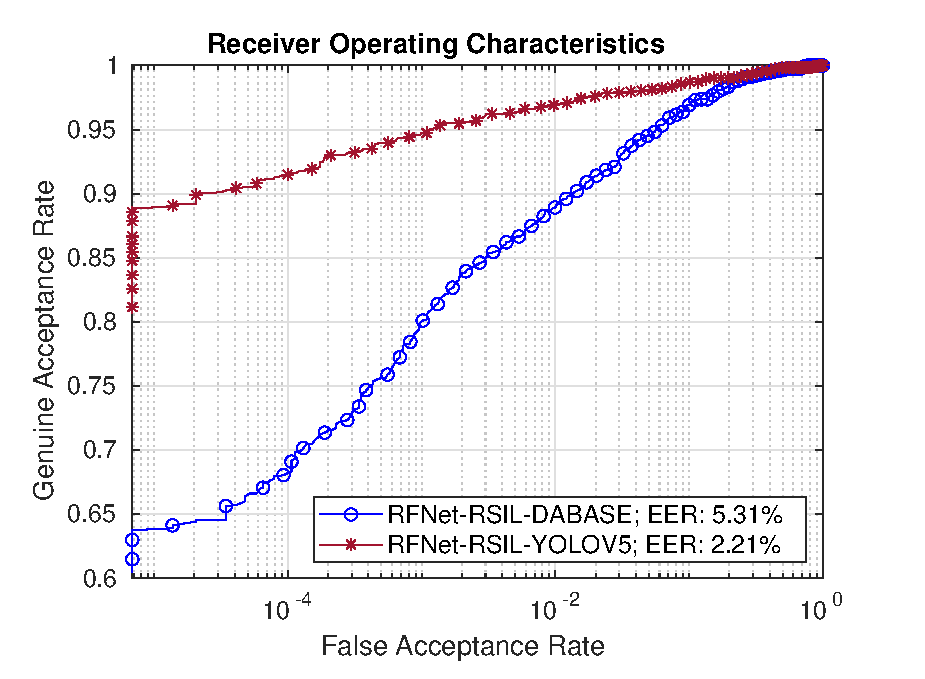
\includegraphics[width=\linewidth]{Figures/yolov5vsdatabase/fkv3-roc_compare_new.eps}
	\end{subfigure}
	\begin{subfigure}[b]{0.45\linewidth}
		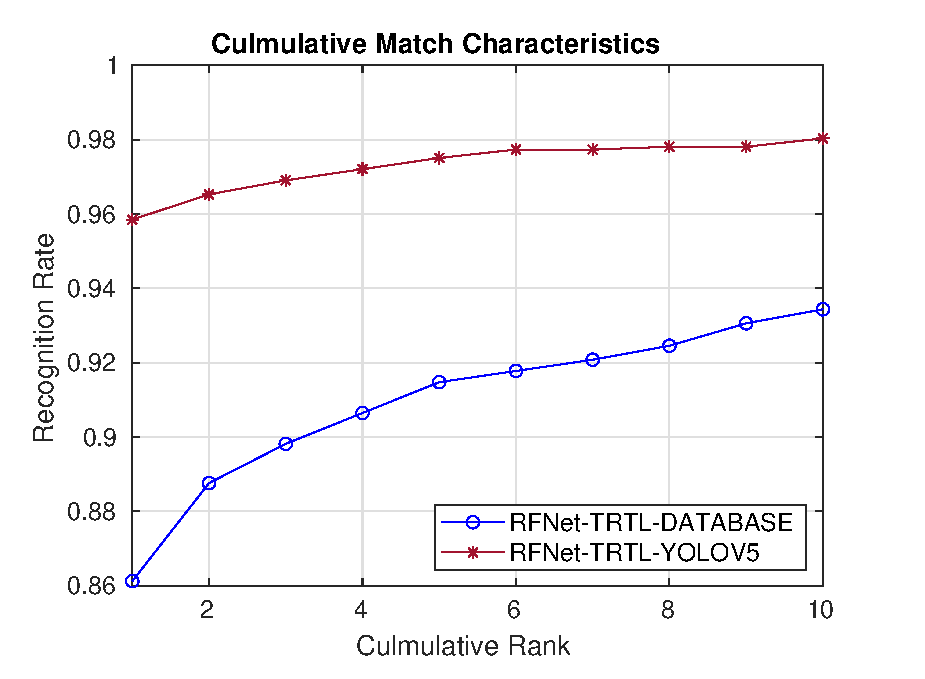
\includegraphics[width=\linewidth]{Figures/yolov5vsdatabase/fkv3-cmc_compare_new.eps}
	\end{subfigure}
	\caption{Compare performance on the Finger Knuckle V3 Dataset (with deformable)}
\end{figure}

\begin{figure}[H]
	\centering
	\begin{subfigure}[b]{0.45\linewidth}
		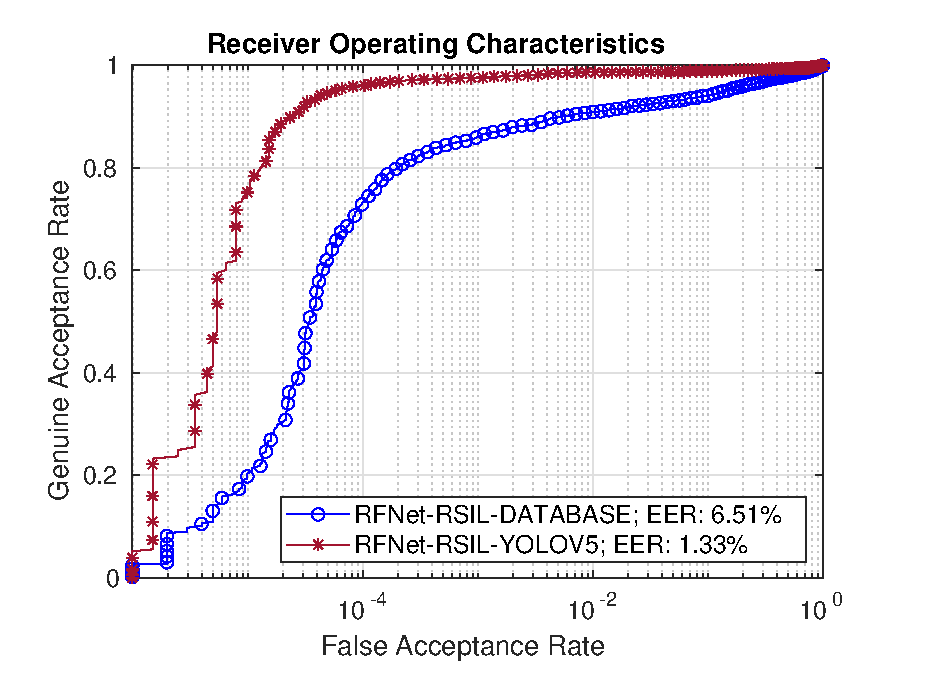
\includegraphics[width=\linewidth]{Figures/yolov5vsdatabase/hd-roc_compare_new.eps}
	\end{subfigure}
	\begin{subfigure}[b]{0.45\linewidth}
		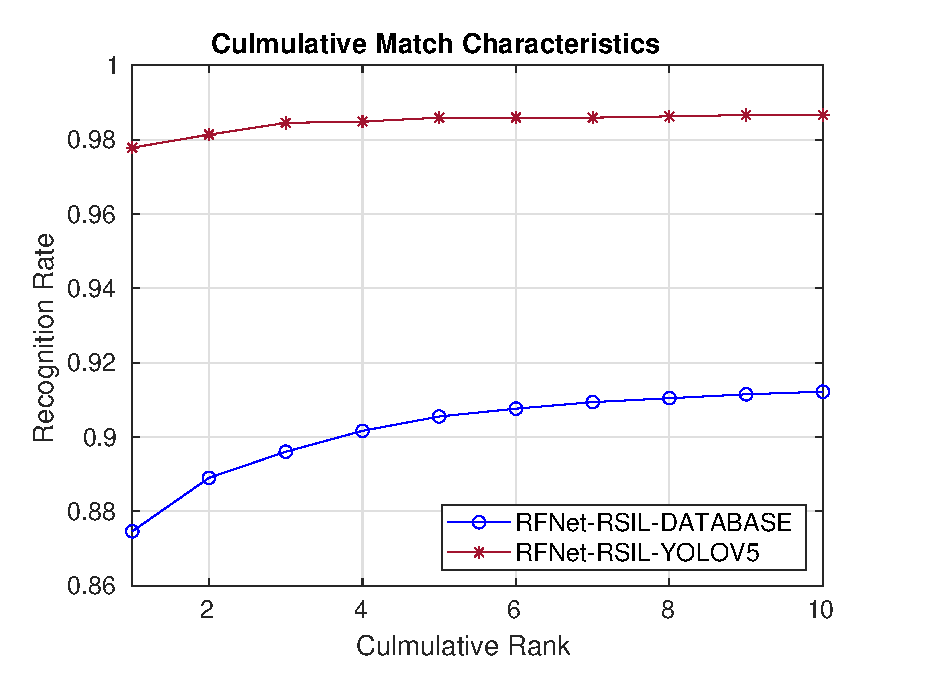
\includegraphics[width=\linewidth]{Figures/yolov5vsdatabase/hd-cmc_compare_new.eps}
	\end{subfigure}
	\caption{Compare performance on the Index Finger of the Hand Dorsal Image Database.}
\end{figure}

From the above ROC curve and ROC curve, we can clearly get the conclusion that quality of segmented finger knuckle of YOLOv5s-CSL is better than the segmented finger knuckle of dataset. When using YOLOv5x-CSL to segment finger knuckle, both of verification performance and recognition performance can increase. Especially on the Hand Dorsal Image Database, the EER value can drop from $6.51\%$ to $1.33\%$, and on the CMC curve, the recognition rate of top 1 can increase from about $87.8\%$ to $97.9\%$.


\subsection{Online Contactless Finger Knuckle Identification Performance}

For proving our contactless and online finger knuckle identification performance, we capture 52 subjects and each subject can offer about 15-20s contactless finger knuckle video using smartphone. The minimum frame rate of the videos that we offer is 30 frames per second. When we capture these finger knuckle videos, we take into account practical application scenarios, therefore, each subject is on a complex background with traffic flow and pedestrian interference. And the finger knuckle rotate from 0 to 180 degrees and the distance from the camera changes, even capturing finger knuckle flexion scenes as well.
  
We choose two method to get the contactless finger knuckle images, one is that we get 1 image per second, another one is that we get 6 images per second for testing online matching performance. Because the shortest video is 15s, for 1 image per second, we can totally get $52*15 = 780$ finger knuckle images for keeping the same number of samples result in $52*15 =1789 $ genuine matching scores and $52*51*15 = 39780$ imposter matching scores. In terms of the 6 images per second, we can get $52*15*6=4680$ finger knuckle samples, result in $52*90=4680$ genuine matching scores and $52*51*90=238680$ imposter matching scores. From the below Figure \ref{1S1F} and \ref{1S6F}, the online identification performance is good enough as an online finger knuckle identification system when using the RFNet to extract finger knuckle pattern. Both of them, the EER is lower than $2.00\%$, and the matching accuracy is higher than $93.00$. At the same time, using RSIL loss, the matching performance can be further improved, although not by much.


\begin{figure}[H]
	\centering
	\begin{subfigure}[b]{0.45\linewidth}
		\includegraphics[width=\linewidth]{Figures/online-performance/1s1f-roc_compare_new.eps}
		\caption{}
	\end{subfigure}
	\begin{subfigure}[b]{0.45\linewidth}
		\includegraphics[width=\linewidth]{Figures/online-performance/1s1f-cmc_compare_new.eps}
		\caption{}
	\end{subfigure}
	\caption{Comparative ROC (a) and corresponding CMC (b) with one session protocol for online finger knuckle video dataset with 1 frame image per second.}
	\label{1S1F}
\end{figure}

\begin{figure}[H]
	\centering
	\begin{subfigure}[b]{0.45\linewidth}
		\includegraphics[width=\linewidth]{Figures/online-performance/1s6f-roc_compare_new.eps}
		\caption{}
	\end{subfigure}
	\begin{subfigure}[b]{0.45\linewidth}
		\includegraphics[width=\linewidth]{Figures/online-performance/1s6f-cmc_compare_new.eps}
		\caption{}
	\end{subfigure}
	\caption{Comparative ROC (a) and corresponding CMC (b) with one session protocol for online finger knuckle video dataset with 6 frame images per second.}
	\label{1S6F}
\end{figure}